
\documentclass[aspectratio=169]{beamer}

\usepackage[utf8]{inputenc}
\usepackage[T1]{fontenc}
\usepackage[ngerman]{babel}
\usepackage{media9}
\usepackage{graphicx}
\usepackage{booktabs}
\usepackage{listings}
\usepackage{xcolor}
\usepackage{textgreek}
\usepackage[absolute, overlay]{textpos}
\usepackage{hyperref}
\setlength{\TPHorizModule}{\paperwidth}
\setlength{\TPVertModule}{\paperheight}
\TPGrid{1}{1}
\usetheme{Madrid}
\setbeamertemplate{frametitle}{}
\usecolortheme{default}

\definecolor{codegreen}{rgb}{0,0.6,0}
\definecolor{codegray}{rgb}{0.5,0.5,0.5}
\definecolor{codepurple}{rgb}{0.58,0,0.82}
\lstdefinestyle{mystyle}{%
    commentstyle=\color{codegreen},
    keywordstyle=\color{magenta},
    numberstyle=\tiny\color{codegray},
    stringstyle=\color{codepurple},
    basicstyle=\ttfamily\footnotesize,
    breakatwhitespace=false,
    breaklines=true,
    captionpos=b,
    keepspaces=true,
    numbers=left,
    numbersep=5pt,
    showspaces=false,
    showstringspaces=false,
    showtabs=false,
    tabsize=2
}
\lstset{style=mystyle}



% --- METADATA ---
\title{Kollisionsdetektion und -antwort}
\author[Dimitrij Pivovar]{Dimitrij Pivovar}
\institute{16.11.2025}
\date{09.12.2024}

\begin{document}

\setbeamertemplate{footline}{} 
\setbeamertemplate{navigation symbols}{}
\begin{frame}
  \titlepage
\end{frame}


% --- Slide 1 ---
\begin{frame}[fragile]
\begin{textblock}{0.825}(0.108, 0.107)
  \begin{minipage}[b][0.427\paperheight]{\linewidth}
    \textbf{Kollisionsdetektion und -antwort}
  \end{minipage}
\end{textblock}

\begin{textblock}{0.821}(0.111, 0.71)
  \begin{minipage}[t][0.213\paperheight]{\linewidth}
    {\small SSDS 24/25 Kurilin, Pivovar}
  \end{minipage}
\end{textblock}
\end{frame}

% --- Slide 2 ---
\begin{frame}[fragile]
\begin{textblock}{0.812}(0.112, 0.043)
  \begin{minipage}[t][0.151\paperheight]{\linewidth}
    \textbf{Inhaltsverzeichnis}
  \end{minipage}
\end{textblock}

\begin{textblock}{0.798}(0.112, 0.338)
  \begin{minipage}[t][0.537\paperheight]{\linewidth}
    {\scriptsize
    \begin{itemize}
      \item Was ist Kollisionsdetektion?
      \item Line of Action
      \item Zentraler elastischer Stoß
      \item Rotation
      \item Probleme bei Kollisionsdetektion
      \item Algorithmen
    \end{itemize}
    }
  \end{minipage}
\end{textblock}

\begin{textblock}{0.225}(0.736, 0.941)
  \begin{minipage}[b][0.053\paperheight]{\linewidth}
    \raggedright
    \fontsize{3}{3.3}\selectfont 16.11.2025
  \end{minipage}
\end{textblock}

\begin{textblock}{0.037}(0.96, 0.941)
  \begin{minipage}[b][0.053\paperheight]{\linewidth}
    \raggedright
    \fontsize{3}{3.3}\selectfont 2
  \end{minipage}
\end{textblock}
\end{frame}

% --- Slide 3 ---
\begin{frame}[fragile]
  \begin{textblock}{0.437}(0.093, 0.073)
    \begin{minipage}[t][0.24\paperheight]{\linewidth}
      \textbf{Kollisionsdetektion bei balls2D}
    \end{minipage}
  \end{textblock}
  \begin{textblock}{0.436}(0.094, 0.351)
    \begin{minipage}[t][0.515\paperheight]{\linewidth}
      {\small Gehen über alle Bälle, berechnen die Distanz zwischen den Bällen und wenn die Distanz kleiner ist als die Summe beider Radien dann wird eine Kollision erkannt}
    \end{minipage}
  \end{textblock}
  \begin{textblock}{0.225}(0.735, 0.942)
    \begin{minipage}[b][0.053\paperheight]{\linewidth}
      \raggedright
      \fontsize{3}{3.3}\selectfont 16.11.2025
    \end{minipage}
  \end{textblock}
  \begin{textblock}{0.037}(0.96, 0.942)
    \begin{minipage}[b][0.053\paperheight]{\linewidth}
      \raggedright
      \fontsize{3}{3.3}\selectfont 3
    \end{minipage}
  \end{textblock}
  \begin{textblock}{0.449}(0.553, 0.351)
    \begin{minipage}[t][0.381\paperheight]{\linewidth}
      
\includegraphics[width=\linewidth,height=\textheight,keepaspectratio]{extracted_media/image_1.png}
    \end{minipage}
  \end{textblock}
  \begin{textblock}{0.449}(0.553, 0.351)
    \begin{minipage}[t][0.381\paperheight]{\linewidth}
      
\includegraphics[width=\linewidth,height=\textheight,keepaspectratio]{extracted_media/image_1.png}
    \end{minipage}
  \end{textblock}
\end{frame}

% --- Slide 4 ---
\begin{frame}[fragile]
  \begin{textblock}{0.437}(0.093, 0.073)
    \begin{minipage}[t][0.24\paperheight]{\linewidth}
      \textbf{Was ist Kollisionsantwort?}
    \end{minipage}
  \end{textblock}
  \begin{textblock}{0.436}(0.094, 0.351)
    \begin{minipage}[t][0.515\paperheight]{\linewidth}
      {\small
        Wenn eine Kollision erkannt wird, muss diese aufgelöst werden. Das gelingt dadurch das man die Positionen der Bälle auflöst, einen neuen Bewegungsvektor berechnet und eine neue Velocity berechnet mit der die Bälle in die Richtung des neuen Bewegungsvektors bewegt werden
      }
    \end{minipage}
  \end{textblock}
  \begin{textblock}{0.225}(0.735, 0.942)
    \begin{minipage}[b][0.053\paperheight]{\linewidth}
      \raggedright
      \fontsize{3}{3.3}\selectfont 16.11.2025
    \end{minipage}
  \end{textblock}
  \begin{textblock}{0.037}(0.96, 0.942)
    \begin{minipage}[b][0.053\paperheight]{\linewidth}
      \raggedright
      \fontsize{3}{3.3}\selectfont 4
    \end{minipage}
  \end{textblock}
  \begin{textblock}{0.342}(0.58, 0.28)
    \begin{minipage}[t][0.445\paperheight]{\linewidth}
      
\includegraphics[width=\linewidth, height=\textheight, keepaspectratio]{extracted_media/image_2.png}
    \end{minipage}
  \end{textblock}
\end{frame}

% --- Slide 5 ---
\begin{frame}[fragile]
\begin{textblock}{0.236}(0.054, 0.403)
  \begin{minipage}[t][0.448\paperheight]{\linewidth}
    \textbf{Abfragen bei Quadtree}
  \end{minipage}
\end{textblock}
\begin{textblock}{0.225}(0.736, 0.941)
  \begin{minipage}[b][0.053\paperheight]{\linewidth}
    \raggedright
    \fontsize{3}{3.3}\selectfont 11/16/2025
  \end{minipage}
\end{textblock}
\begin{textblock}{0.037}(0.96, 0.941)
  \begin{minipage}[b][0.053\paperheight]{\linewidth}
    \raggedright
    \fontsize{3}{3.3}\selectfont 5
  \end{minipage}
\end{textblock}
\begin{textblock}{0.593}(0.369, 0.204)
  \begin{minipage}[t][0.593\paperheight]{\linewidth}
    \includemedia[
       width=\linewidth, 
       height=0.593\paperheight,
       activate=pageopen, 
       addresource=extracted_media/media_3.mp4, 
       flashvars={
          source=extracted_media/media_3.mp4 
          &autoPlay=true 
          &loop=true
       }
    ]{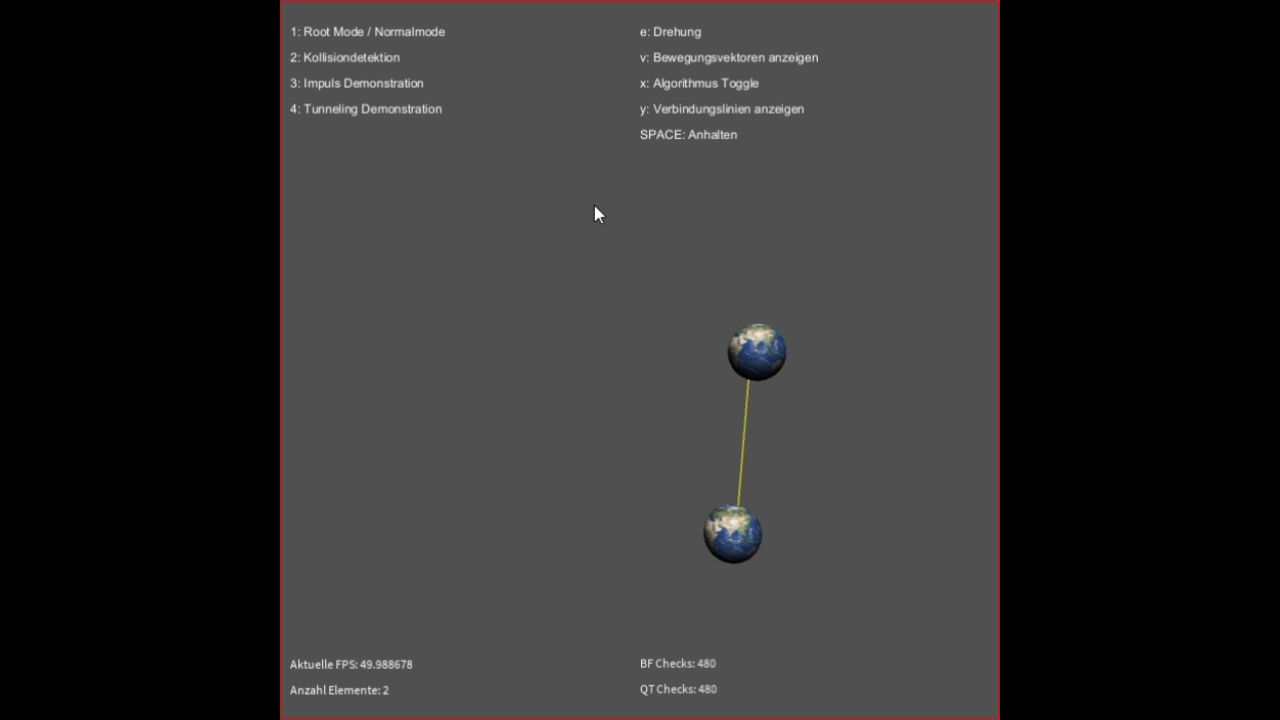
\includegraphics[width=\linewidth,height=\textheight]{extracted_media/media_3_poster.png}}{VPlayer.swf}
  \end{minipage}
\end{textblock}
\end{frame}

% --- Slide 6 ---
\begin{frame}[fragile]
  \begin{textblock}{0.347}(0.068, 0.086)
    \begin{minipage}[t][0.494\paperheight]{\linewidth}
      \textbf{Fragen?}
    \end{minipage}
  \end{textblock}

  \begin{textblock}{0.399}(0.533, 0.095)
    \begin{minipage}[t][0.809\paperheight]{\linewidth}
      {\small
        Vielen Dank für Ihre Aufmerksamkeit
      }
    \end{minipage}
  \end{textblock}

  \begin{textblock}{0.225}(0.736, 0.941)
    \begin{minipage}[b][0.053\paperheight]{\linewidth}
      \raggedright
      \fontsize{3}{3.3}\selectfont 16.11.2025
    \end{minipage}
  \end{textblock}

  \begin{textblock}{0.037}(0.96, 0.941)
    \begin{minipage}[b][0.053\paperheight]{\linewidth}
      \raggedright
      \fontsize{3}{3.3}\selectfont 6
    \end{minipage}
  \end{textblock}
\end{frame}

% --- Slide 7 ---
\begin{frame}[fragile]
  \begin{textblock}{0.812}(0.112, 0.043)
    \begin{minipage}[t][0.151\paperheight]{\linewidth}
      \textbf{Quellen}
    \end{minipage}
  \end{textblock}
  
  \begin{textblock}{0.798}(0.112, 0.338)
    \begin{minipage}[t][0.537\paperheight]{\linewidth}
      \scriptsize
      \begin{itemize}
        \item https://www.leifiphysik.de/mechanik/impulserhaltung-und-stoesse/aufgabe/geschwindigkeiten-nach-einem-zentralen-elastischen-stoss
        \item https://www.leifiphysik.de/mechanik/kreisbewegung/grundwissen/bahngeschwindigkeit-und-winkelgeschwindigkeit
        \item https://www.mdpi.com/applsci/applsci-10-07636/article_deploy/html/images/applsci-10-07636-g001.png
        \item https://gamedev.stackexchange.com/questions/192400/in-games-physics-engines-what-is-tunneling-also-known-as-the-bullet-through
      \end{itemize}
    \end{minipage}
  \end{textblock}

  \begin{textblock}{0.225}(0.736, 0.941)
    \begin{minipage}[b][0.053\paperheight]{\linewidth}
      \raggedright
      \fontsize{3}{3.3}\selectfont 16.11.2025
    \end{minipage}
  \end{textblock}

  \begin{textblock}{0.037}(0.96, 0.941)
    \begin{minipage}[b][0.053\paperheight]{\linewidth}
      \raggedright
      \fontsize{3}{3.3}\selectfont 7
    \end{minipage}
  \end{textblock}
\end{frame}


\end{document}
